% Name: Mean value theorem
% Description: The secant from A to B and the two points c₁ and c₂ between them where the tangent is parallel to it, so f′(c) equals the average slope.
% Tags: mean value theorem, secant, tangent, derivative

\usetikzlibrary{arrows.meta}

\begin{tikzpicture}[>={Stealth}, yscale=1.4, every node/.style={font=\small}]
  \draw[->] (-0.2,0) -- (6.3,0) node[right] {$x$};
  \draw[->] (0,-0.2) -- (0,3.4) node[above] {$y$};
  \draw[very thick, blue!70!black, domain=0.2:5.9, samples=80, smooth] plot (\x, {0.1*\x^3 - 0.9*\x^2 + 2.2*\x + 1}) node[right] {$f$};
  % f(0.5) = 1.8875 and f(5.5) = 2.5125, so the secant's slope is 0.125; f'(c) = 0.3c² - 1.8c + 2.2 = 0.125 gives c = 3 ± √(1.0833) ≈ 1.557 and 4.443
  \draw[thick, orange!85!black] (0.5,1.8875) -- (5.5,2.5125);
  \foreach \c/\y/\n in {1.557/2.621/1, 4.443/1.779/2} {
    \draw[thick, green!50!black] (\c-1.1,\y-0.1375) -- (\c+1.1,\y+0.1375);
    \draw[dashed, gray] (\c,\y) -- (\c,0) node[below, black] {$c_\n$};
    \fill[green!50!black] (\c,\y) circle (1.6pt);
  }
  \foreach \x/\y/\p in {0.5/1.8875/A, 5.5/2.5125/B} {
    \draw[dashed, gray] (\x,\y) -- (\x,0);
    \fill (\x,\y) circle (1.8pt) node[above left] {$\p$};
  }
  \node[below] at (0.5,0) {$a$};
  \node[below] at (5.5,0) {$b$};
  \node at (3,-0.75) {$f'(c) = \dfrac{f(b) - f(a)}{b - a}$};
\end{tikzpicture}
